\documentclass[10pt,compress,t,notes=noshow,xcolor=table]{beamer}

\input{../../style/preamble}
\input{../../latex-math/basic-math}
\input{../../latex-math/basic-ml}

\usepackage{tikz}
\usetikzlibrary{arrows.meta, positioning, calc, decorations.pathreplacing}

\title{Interpretable Machine Learning}

\begin{document}

\titlemeta{
Feature Effects
}{
ALE Walkthrough: Bike Sharing Example
}{
figure/ale_plot.pdf
}{
\item Step-by-step: partition, finite differences, average, accumulate, and center
}

% ------------------------------------------------------------
\begin{framev}[align=top]{Formula Recap: What ALE Estimates}
The formula for the \textbf{uncentered} first-order ALE at a specific point $x$ is:
\spacer[0.5]
$$
\hat{\tilde{f}}_{S, \text{ALE}}(x) = \underbrace{ \sum_{k = 1}^{k_S(x)} }_{\text{\parbox{1.5cm}{\centering \textcolor{purple}{Step 4:\\ Accumulate}}}} \underbrace{ \frac{1}{n_S(k)} \sum_{i: \; x_S^{(i)} \in \; \text{int } k} }_{\text{\parbox{2cm}{\centering \textcolor{orange}{Step 3:\\ Local Average}}}} \underbrace{ [\fh(z_{k, S}, \xv_{-S}^{(i)}) -\fh(z_{k-1, S}, \xv_{-S}^{(i)})] }_{\text{\parbox{3cm}{\centering \textcolor{blue}{Step 1 \& 2:\\ Partition \& Finite Diff.}}}}
$$
\spacer[0.5]
\begin{itemizeM}
\item Dataset: bike rentals with features such as temperature, humidity, windspeed, season, weekday, etc.
\item Model:
$$
\hat f(\text{temp}, \text{humidity}, \text{windspeed})
=
\text{predicted number of rented bikes}
$$
\item \textbf{Our Goal:} Explain the effect of \textbf{Temperature} ($x_S$) on the predicted number of rented bikes ($\hat{f}$), while keeping the interactions with Humidity and Windspeed ($\xv_{-S}$) true to the data distribution.
\end{itemizeM}
\end{framev}


% ------------------------------------------------------------
\begin{framev}[align=top]{Step 1: Partition the Feature Range}
\begin{itemizeM}
% \item First, we must divide the continuous feature of interest into $K$ intervals.
\item Suppose temperature ranges from $0^\circ\text{C}$ to $40^\circ\text{C}$ in our training data.
\item For this example, we split the feature space into $K=40$ equidistant intervals of width $1^\circ\text{C}$ ($[0,1), [1,2), \dots, [39,40)$).
\end{itemizeM}
\spacer[0.5]
\begin{center}
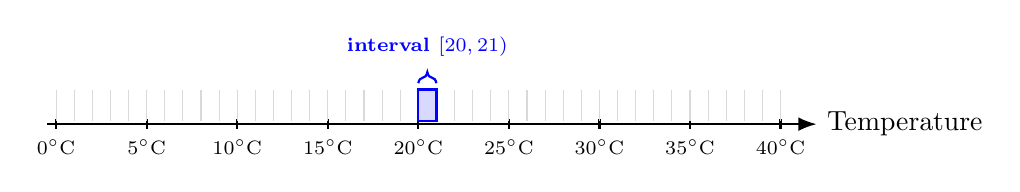
\begin{tikzpicture}[x=0.23cm,y=0.8cm,>=Latex]
\draw[->,thick] (-0.5,0) -- (42,0) node[right] {Temperature};
\foreach \x in {0,5,...,40}{
\draw[thick] (\x,0.08) -- (\x,-0.08) node[below] {\scriptsize \x$^\circ$C};
}
\foreach \x in {0,...,40}{
\draw[gray!30] (\x,0.05) -- (\x,0.55);
}
% Highlight the interval
\draw[fill=blue!15,draw=blue,thick] (20,0.05) rectangle (21,0.55);
% Properly spaced brace and text
\draw[decorate,decoration={brace,amplitude=4pt},blue,thick]
(20,0.65) -- (21,0.65) node[midway,above=6pt, font=\scriptsize\bfseries] {interval $[20,21)$};
\end{tikzpicture}
\end{center}
\spacer[0.5]
\begin{itemizeM}
\item Let's zoom in on the $k$-th interval: \textbf{$[20^\circ\text{C}, 21^\circ\text{C})$}.
\item \textit{Note:} Equidistant intervals preserve resolution, but quantile-based intervals may be used to ensure a balanced number of samples per interval.
\end{itemizeM}
\end{framev}


% ------------------------------------------------------------
\begin{framev}[align=top]{Step 2: Calculate Finite Differences}
\textbf{What happens to the prediction when we cross an interval?}
\spacer[0.2]
\splitVTT[0.45]{
% --- LEFT COLUMN: CONCISE EXPLANATION ---
\spacer[0.6]
\begin{itemizeM}
\item<1-> \textbf{1. Select:} Find a data point that falls into the interval (e.g., $obs_A$ at $20.5^\circ\text{C}$).
\spacer[0.25]
\item<2-> \textbf{2. Substitute:} Replace its temperature with the lower ($20$) and upper ($21$) interval bounds.\\
\textcolor{gray}{\scriptsize \textit{Crucial: Keep all other features exactly as observed!}}
\spacer[0.25]
\item<3-> \textbf{3. Calculate:} Predict the outcomes for both new points and subtract to isolate the \textbf{local effect}.
\end{itemizeM}
}{
% --- RIGHT COLUMN: TIKZ FIGURE ---
\spacer[0]
\centering
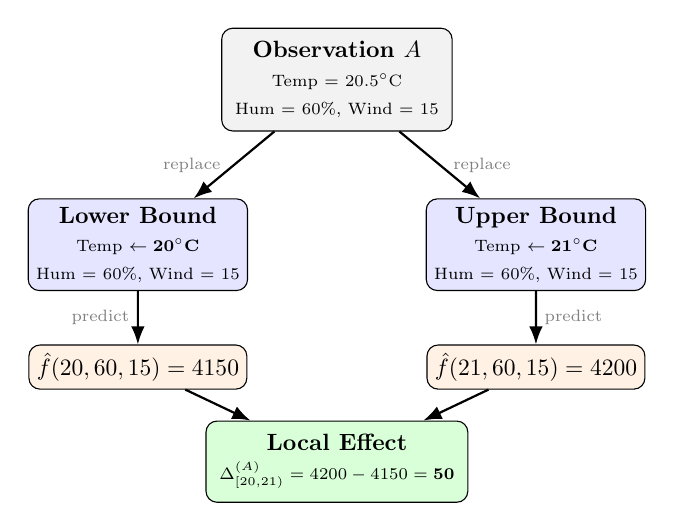
\begin{tikzpicture}[>=Latex, node distance=1.2cm and 0.1cm, scale=0.85, transform shape]
% Step 1: Initial Observation
\node<1->[draw, fill=gray!10, rounded corners, align=center, inner sep=2mm] (obs)
{\textbf{Observation $A$}\\ \scriptsize Temp = $20.5^\circ$C\\ \scriptsize Hum = $60\%$, Wind = $15$};
% Step 2: Branching to bounds
\node<2->[draw, fill=blue!10, rounded corners, align=center, below left=1cm and -0.4cm of obs] (lo)
{\textbf{Lower Bound}\\ \scriptsize Temp $\leftarrow \mathbf{20^\circ\text{C}}$\\ \scriptsize Hum = $60\%$, Wind = $15$};
\node<2->[draw, fill=blue!10, rounded corners, align=center, below right=1cm and -0.4cm of obs] (hi)
{\textbf{Upper Bound}\\ \scriptsize Temp $\leftarrow \mathbf{21^\circ\text{C}}$\\ \scriptsize Hum = $60\%$, Wind = $15$};
\draw<2->[->, thick] (obs) -- (lo) node[midway, left=2pt, font=\scriptsize, text=gray] {replace};
\draw<2->[->, thick] (obs) -- (hi) node[midway, right=2pt, font=\scriptsize, text=gray] {replace};
% Step 3: Predictions
\node<3->[draw, fill=orange!10, rounded corners, below=0.8cm of lo] (predlo)
{$\hat{f}(20, 60, 15) = 4150$};
\node<3->[draw, fill=orange!10, rounded corners, below=0.8cm of hi] (predhi)
{$\hat{f}(21, 60, 15) = 4200$};
\draw<3->[->, thick] (lo) -- (predlo) node[midway, left, font=\scriptsize, text=gray] {predict};
\draw<3->[->, thick] (hi) -- (predhi) node[midway, right, font=\scriptsize, text=gray] {predict};
% Step 3: Difference (Dynamically anchored below the prediction nodes)
\coordinate<3-> (midpred) at ($(predlo)!0.5!(predhi)$);
\node<3->[draw, fill=green!15, rounded corners, below=0.8cm of midpred, inner sep=2mm, align=center] (diff)
{\textbf{Local Effect}\\ \scriptsize $\Delta^{(A)}_{[20,21)} = 4200 - 4150 = \mathbf{50}$};
\draw<3->[->, thick] (predlo) -- (diff);
\draw<3->[->, thick] (predhi) -- (diff);
\end{tikzpicture}
}
\end{framev}


% ------------------------------------------------------------
\begin{framev}[align=top]{Step 3: Local Averaging}
$$
\textcolor{orange}{\bar{\Delta}_{[20,21)} = \frac{1}{n_{[20,21)}} \sum_{i:\;x_{\text{temp}}^{(i)}\in[20,21)}} [\Delta^{(i)}_{[20,21)}]
$$
\begin{itemizeM}
\item We repeat Step 2 for \textbf{every} observation located inside the $[20,21)$ interval.
\item Because each observation has unique background features (humidity, windspeed), their individual local effects ($\Delta^{(i)}$) may vary.
\end{itemizeM}
\spacer[0.25]
\begin{center}
\rowcolors{2}{gray!8}{white}
\begin{tabular}{c c c c}
\toprule
\textbf{Observation} & \textbf{Humidity} & \textbf{Windspeed} & \textbf{Finite Difference ($\Delta$)} \\
\midrule
$obs_A$ & $60\%$ & $15$ km/h & $50$ bikes \\
$obs_B$ & $64\%$ & $11$ km/h & $44$ bikes \\
$obs_C$ & $58\%$ & $18$ km/h & $62$ bikes \\
$obs_D$ & $70\%$ & $13$ km/h & $54$ bikes \\
\bottomrule
\end{tabular}
\end{center}
\spacer[0.25]
\begin{itemizeM}
\item By averaging these, we estimate the expected local effect: $\bar{\Delta}_{[20,21)} = \mathbf{52.5}$.
\end{itemizeM}
\end{framev}


% ------------------------------------------------------------
\begin{framev}[align=top]{Step 4: Accumulate Local Effects}
$$
\hat{\tilde f}_{\text{temp},\text{ALE}}(x) = \textcolor{purple}{\sum_{k=1}^{k(x)}} \bar\Delta_k
$$
To find the uncentered ALE effect at $x = 21^\circ\text{C}$, we must \textbf{accumulate} (sum) all the average local effects from the minimum temperature up to $21^\circ\text{C}$.
\spacer[0.3]
\begin{center}
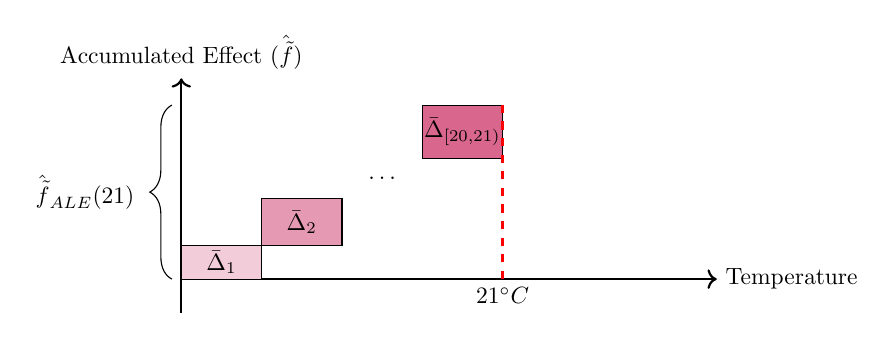
\begin{tikzpicture}[scale=0.85, every node/.style={scale=0.85}]
% Axes
\draw[->, thick] (0,0) -- (8,0) node[right] {Temperature};
\draw[->, thick] (0,-0.5) -- (0,3) node[above] {Accumulated Effect ($\hat{\tilde{f}}$)};
% Bars to show accumulation
\draw[fill=purple!20] (0,0) rectangle (1.2, 0.5);
\node at (0.6, 0.25) {$\bar{\Delta}_1$};
\draw[fill=purple!40] (1.2,0.5) rectangle (2.4, 1.2);
\node at (1.8, 0.85) {$\bar{\Delta}_2$};
\node at (3.0, 1.5) {$\dots$};
\draw[fill=purple!60] (3.6, 1.8) rectangle (4.8, 2.6);
\node at (4.2, 2.2) {$\bar{\Delta}_{[20,21)}$};
% Target line
\draw[thick, dashed, red] (4.8,0) -- (4.8, 2.6);
\node[below] at (4.8,0) {$21^\circ\text{C}$};
% Bracket showing the sum
\draw[decorate, decoration={brace, amplitude=8pt}, xshift=-4pt, yshift=0pt]
(0,0) -- (0,2.6) node [black, midway, xshift=-1.3cm] {$\hat{\tilde{f}}_{\text{ALE}}(21)$};
\end{tikzpicture}
\end{center}
\end{framev}


% ------------------------------------------------------------
\begin{framev}[align=top]{Step 5: Centering}
$$
\hat f_{\text{temp},\text{ALE}}(x) = \hat{\tilde f}_{\text{temp},\text{ALE}}(x) - \underbrace{ \frac{1}{n} \sum_{i=1}^{n} \hat{\tilde f}_{\text{temp},\text{ALE}} (x_{\text{temp}}^{(i)}) }_{\text{Mean shift } (c)}
$$
Centering shifts the curve so the average effect across the dataset is $0$.
\spacer[0.25]
\begin{center}
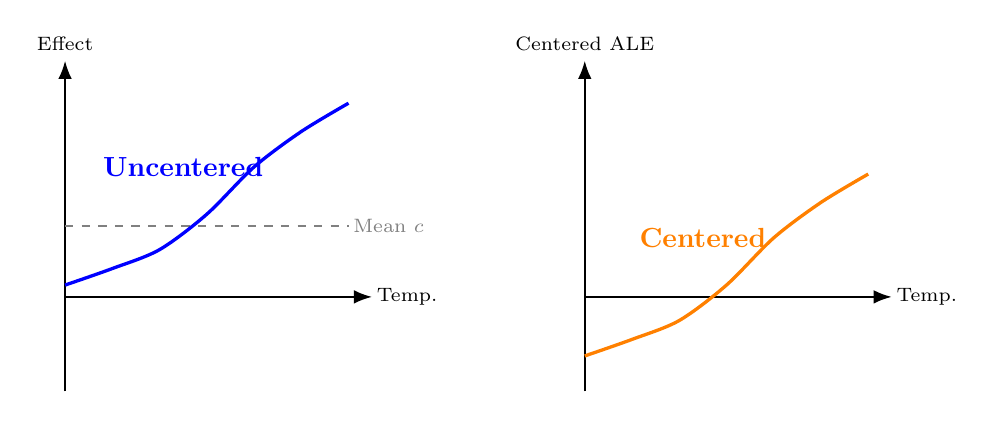
\begin{tikzpicture}[x=0.6cm, y=0.03cm, >=Latex, font=\scriptsize]
% Uncentered
\draw[->,thick] (0,0) -- (6.5,0) node[right=-2pt] {Temp.};
\draw[->,thick] (0,-40) -- (0,100) node[above] {Effect};
\draw[gray,dashed,thick] (0,30) -- (6,30) node[right=-2pt] {Mean $c$};
\draw[blue,very thick] plot[smooth] coordinates {(0,5) (1,12) (2,20) (3,35) (4,55) (5,70) (6,82)};
\node[blue, font=\bfseries] at (2.5, 55) {Uncentered};
% Arrow
%   \draw[thick, ->, bend left=15] (7.5, 30) to node[midway, above=4pt, align=center] {Shift by $c$\\to center at $0$} (9.5, 30);
% Centered
\begin{scope}[shift={(11,0)}]
\draw[->,thick] (0,0) -- (6.5,0) node[right=-2pt] {Temp.};
\draw[->,thick] (0,-40) -- (0,100) node[above] {Centered ALE};
%   \draw[gray,dashed,thick] (0,0) -- (6,0) node[right=-2pt] {Zero};
\draw[orange,very thick] plot[smooth] coordinates {(0,-25) (1,-18) (2,-10) (3,5) (4,25) (5,40) (6,52)};
\node[orange, font=\bfseries] at (2.5, 25) {Centered};
\end{scope}
\end{tikzpicture}
\end{center}
\end{framev}


% ------------------------------------------------------------
\begin{framev}[align=top]{Complete Walkthrough in One Picture}
\begin{enumerate}[<+->]
\item Partition temperature into intervals:
$$
[0,1),[1,2),\ldots,[39,40)
$$
\item For each observation in an interval, replace temperature by both interval boundaries:
$$
\hat f(z_k,\xv_{-\text{temp}}^{(i)})
-
\hat f(z_{k-1},\xv_{-\text{temp}}^{(i)})
$$
\item Average these differences within the interval:
$$
\bar\Delta_k
=
\frac{1}{n_k}
\sum_{i:\;x_{\text{temp}}^{(i)}\in[z_{k-1},z_k)}
[
\hat f(z_k,\xv_{-\text{temp}}^{(i)})
-
\hat f(z_{k-1},\xv_{-\text{temp}}^{(i)})
]
$$
\item Accumulate:
$$
\hat{\tilde f}_{\text{temp},\text{ALE}}(z_m)
=
\sum_{k=1}^{m}\bar\Delta_k
$$
\item Center:
$$
\hat f_{\text{temp},\text{ALE}}(x)
=
\hat{\tilde f}_{\text{temp},\text{ALE}}(x)
-
\frac{1}{n}
\sum_{i=1}^{n}
\hat{\tilde f}_{\text{temp},\text{ALE}}(x_{\text{temp}}^{(i)})
$$
\end{enumerate}
\end{framev}


% ------------------------------------------------------------
\begin{framev}[align=top]{Key Intuition}
\begin{itemizeM}
\item \textbf{Finite difference:} “What happens if we move temperature across this small interval?”
\item \textbf{Local averaging:} “Average only over observations that actually live in this temperature region.”
\item \textbf{Accumulation:} “Add up these small local effects to recover the global temperature effect.”
\item \textbf{Centering:} “Shift the curve so that it has mean zero.”
\end{itemizeM}
\end{framev}

\endlecture
\end{document}
